\documentclass{article}
\usepackage[T1]{fontenc}
\usepackage{lmodern}
\usepackage{graphicx}
\usepackage{amsmath,amssymb}
\usepackage[a4paper,margin=2cm]{geometry}
\usepackage[absolute,overlay]{textpos}
\setlength{\TPHorizModule}{1mm}
\setlength{\TPVertModule}{1mm}
\usepackage[indonesian]{babel}
\usepackage{hyperref}
\setlength{\emergencystretch}{2em}
% unit: Halaman 36

\begin{document}

% === Halaman 36 (llm) ===

\begin{itemize}
  \item Nilai $kP$ untuk $k = 2, 3, \dots$ diperlihatkan pada tabel:
\end{itemize}

\vspace{10mm}

Jika diketahui $P$, maka kita bisa menghitung
\[ Q = kP \]

Jika persoalannya dibalik sbb:
\textcolor{red}{Diberikan $P$ dan $Q$, maka sangat sukar menghitung $k$ sedemikian sehingga $Q = kP$}

\begin{center}
  $\Downarrow$ \\
  \textbf{ECDLP}
\end{center}

% deskripsi: Tabel yang menunjukkan nilai k dan hasil kP untuk nilai k dari 1 sampai 13
% bbox normalisasi: [0.2050, 0.1710, 0.3420, 0.9170]
\begin{textblock*}{28.77mm}(43.05mm,50.79mm)
\noindent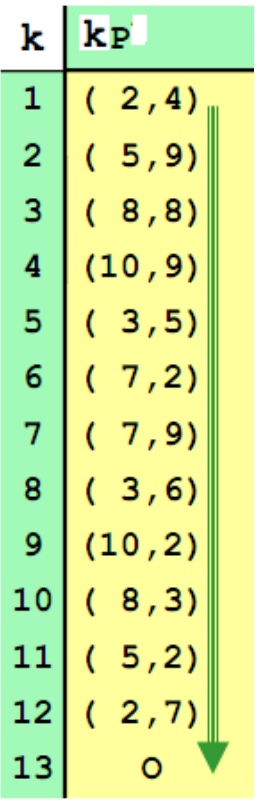
\includegraphics[width=28.77mm,height=221.56mm]{../../images/llm/page_036_img_01.png}%
\end{textblock*}

\end{document}
